% Template from https://www.overleaf.com/latex/templates/ieee-conference-template/grfzhhncsfqn
\documentclass[conference]{IEEEtran}
\IEEEoverridecommandlockouts
% The preceding line is only needed to identify funding in the first footnote. If that is unneeded, please comment it out.
\usepackage{cite}
\usepackage{amsmath,amssymb,amsfonts}
\usepackage{algorithmic}
\usepackage{graphicx}
\usepackage{textcomp}
\usepackage{xcolor}
\def\BibTeX{{\rm B\kern-.05em{\sc i\kern-.025em b}\kern-.08em
    T\kern-.1667em\lower.7ex\hbox{E}\kern-.125emX}}
\begin{document}

\title{Vehicle-to-Vehicle (V2V) Communication Implementation\\
\thanks{University of Florida}
}

\author{
    \IEEEauthorblockN{Gunnar Fandrich}
    \IEEEauthorblockA{
        \textit{Group: Autogators} \\
        \textit{Electrical and Computer Engineering} \\
        \textit{University of Florida} \\
Gainesville, Florida \\
todo@ufl.edu
    }
    \and
    \IEEEauthorblockN{Mark Lai}
    \IEEEauthorblockA{
        \textit{Group: Autogators} \\
        \textit{Electrical and Computer Engineering} \\
        \textit{University of Florida} \\
Gainesville, Florida \\
todo@ufl.edu
    }
    \and
    \IEEEauthorblockN{Rafael Hernandez-Lopez}
    \IEEEauthorblockA{
        \textit{Group: Autogators} \\
        \textit{Electrical and Computer Engineering} \\
        \textit{University of Florida} \\
Gainesville, Florida \\
rhernandezlopez1@ufl.edu
    }
    \and
    \IEEEauthorblockN{Rohan Malik}
    \IEEEauthorblockA{
        \textit{Group: Autogators} \\
        \textit{Electrical and Computer Engineering} \\
        \textit{University of Florida} \\
Gainesville, Florida \\
todo@ufl.edu
    }
}

\maketitle

\begin{abstract}
Vehicle-to-vehicle (V2V) allows communication between vehicles, promoting driver
awareness and potentially reducing the number of collisions. Existing V2V
implementations (cellular V2X, C-V2X) rely on cloud data, whereas the
implementation shown in this paper does true V2V between vehicles.
\end{abstract}

\begin{IEEEkeywords}
V2V, vehicles, driver, awareness, C, ESP32, UDP
\end{IEEEkeywords}

\section{Introduction}
Various process flows are used by the electronics industry to fabricate
transistors. One of the available nodes for manufacturing FinFET transistors is
the 14 nm process node. This process will be outlined and explained.
Renders from Conventor's SEMulator3D software will be used to illustrate
various steps from the process flow.

The four main steps in 14 nm FinFET manufacturing are wafer setup,
front-end-of-line (FEOL), middle-of-line (MOL), and extract devices according to
Conventor's SEMulator3D. Wafer setup is where the manufacture gets the silicon
ready, FEOL makes the FinFET,  MOL connects to the FinFET, and extract devices
is where the tool slices out the FinFET from the render.

\section{Wafer Setup}

\section{Front-End-of-Line}

\paragraph{LTH Mand} After low-temperature hydrogenation \cite{knekr}, the resist layer will
be etched and expose the SiARC underneath. This results in the stack from
Fig.~\ref{lth_mand}.
TODO: Explain what we use this for.

\begin{figure}[htbp]
\centerline{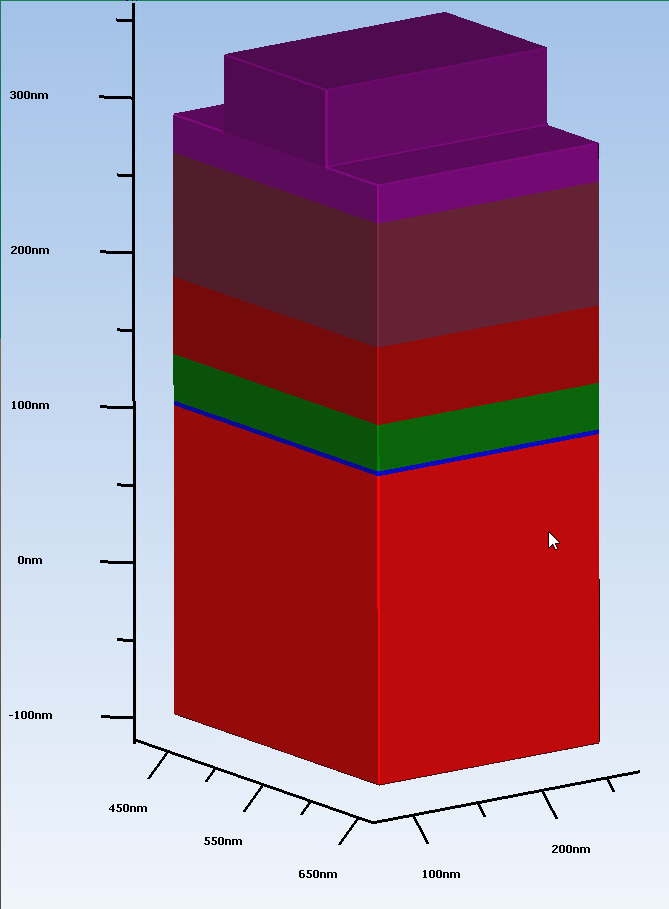
\includegraphics[width=\linewidth]{pics/lth_mand.png}}
\caption{The silicon stack after LTH Mand.}
\label{lth_mand}
\end{figure}

\paragraph{RIE Mand} Reactive ion etching (RIE) \cite{1481759} is used to cut
the SiARC layer, exposing the ODL underneath.

\section{Middle-of-Line}
Explanation on MOL.

\section{Extract Devices}
Explanation on extracting devices.

\section{Conclusion}
Lots of things happen in the 14 nm process flow.

\clearpage
\bibliographystyle{IEEEtran}
\bibliography{bibs}

\end{document}

